% Für die Fehlerrechung wird die empirische Standardabweichung
% \begin{equation}
%   \sigma = \sqrt{\frac{1}{n-1} \cdot \sum_{i=1}^n(x_i-\overline{x})^2}
%   \label{eqn:Stdabweichung}
% \end{equation}
% und die Gaußsche Fehlerfortpflanzung
% \begin{equation}
%   u_y = \sqrt{\sum_{i=1}^n\left(\frac{\delta y}{\delta x_i}u_x\right)^2}
%   \label{eqn:gauß}
% \end{equation}
% verwendet.
% \begin{figure}
%   \centering
%   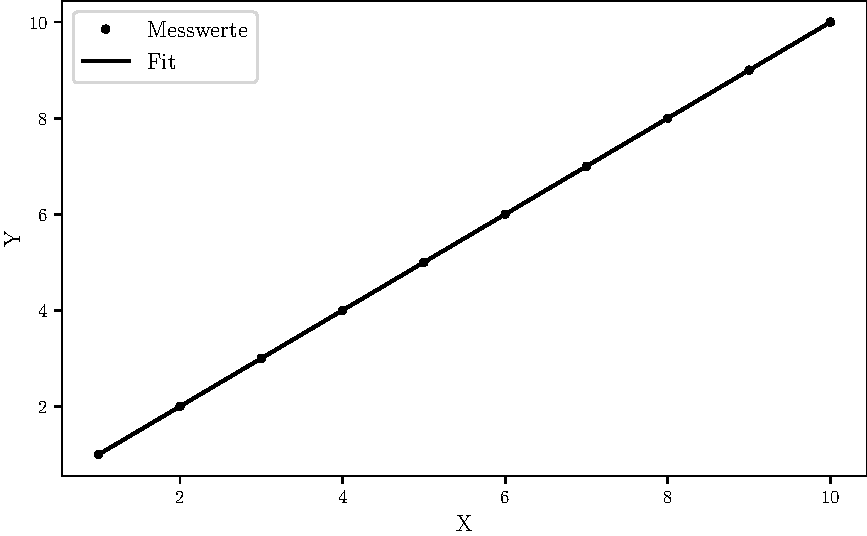
\includegraphics{build/plot.pdf}
%   \caption{Plot}
%   \label{fig:plot}
% \end{figure}
\noindent Die Qualität der Interferenzsignale lässt sich durch den Kontrast $K$
quantifizieren. Um diesen zu ermitteln, wird der initiale Polarisationsfilter
in einem Intervall $\Theta \in [\SI{345}{\degree}, \SI{195}{\degree}]$
in Schritten von je $\theta = \SI{15}{\degree}$ gedreht und die Spannungsmaxima
gemessen. Die Messwerte sind in Tabelle \ref{tabular_01} dargelegt. In den
Bereichen um Winkel, an denen der Kontrast besonders nahe dem Idealwert $K= 1$
liegt, werden zusätzliche Messungen durchgeführt. \\
\FloatBarrier
\begin{table}
  \centering
  \caption{Polarisationsabhängigkeit der Intensitätsextrema.}
  \label{tabular_01}
  \begin{tabular}{c c c c | c c c c}
    \toprule
   \multicolumn{1}{c}{$\Theta$} & \multicolumn{1}{c}{$U_\text{min}$} & \multicolumn{1}{c}{$U_\text{max}$}
    & \multicolumn{1}{c}{$K$} & \multicolumn{1}{c}{$\Theta$} & \multicolumn{1}{c}{$U_\text{min}$}
    & \multicolumn{1}{c}{$U_\text{max}$} & \multicolumn{1}{c}{$K$}\\
   \midrule
   \SI{-15}{\degree} & \SI{694}{\milli\volt} & \SI{1710}{\milli\volt} &  {0.42} & \SI{105}{\degree} & \SI{640}{\milli\volt} & \SI{1572}{\milli\volt} &  {0.42} \\
   \SI{0  }{\degree} & \SI{765}{\milli\volt} & \SI{906 }{\milli\volt} &  {0.08} & \SI{120}{\degree} & \SI{306}{\milli\volt} & \SI{2250}{\milli\volt} &  {0.76} \\
   \SI{15 }{\degree} & \SI{377}{\milli\volt} & \SI{712 }{\milli\volt} &  {0.31} & \SI{130}{\degree} & \SI{200}{\milli\volt} & \SI{2670}{\milli\volt} &  {0.86} \\
   \SI{30 }{\degree} & \SI{148}{\milli\volt} & \SI{620 }{\milli\volt} &  {0.61} & \SI{135}{\degree} & \SI{168}{\milli\volt} & \SI{2540}{\milli\volt} &  {0.88} \\
   \SI{40 }{\degree} & \SI{67 }{\milli\volt} & \SI{696 }{\milli\volt} &  {0.82} & \SI{140}{\degree} & \SI{219}{\milli\volt} & \SI{2640}{\milli\volt} &  {0.85} \\
   \SI{45 }{\degree} & \SI{63 }{\milli\volt} & \SI{740 }{\milli\volt} &  {0.84} & \SI{150}{\degree} & \SI{355}{\milli\volt} & \SI{2270}{\milli\volt} &  {0.73} \\
   \SI{50 }{\degree} & \SI{58 }{\milli\volt} & \SI{770 }{\milli\volt} &  {0.86} & \SI{165}{\degree} & \SI{571}{\milli\volt} & \SI{1514}{\milli\volt} &  {0.45} \\
   \SI{60 }{\degree} & \SI{91 }{\milli\volt} & \SI{951 }{\milli\volt} &  {0.83} & \SI{180}{\degree} & \SI{721}{\milli\volt} & \SI{862 }{\milli\volt} &  {0.09} \\
   \SI{75 }{\degree} & \SI{339}{\milli\volt} & \SI{1167}{\milli\volt} &  {0.55} & \SI{195}{\degree} & \SI{317}{\milli\volt} & \SI{704 }{\milli\volt} &  {0.38} \\
   \SI{90 }{\degree} & \SI{809}{\milli\volt} & \SI{1074}{\milli\volt} &  {0.14} \\
\bottomrule
  \end{tabular}
\end{table}

\FloatBarrier
\noindent Die Spannungsextrema lassen sich dabei anstelle der Intensitätsextrema
in Gleichung \ref{eqn:01} einsetzen, sodass als Kontrast für weitere Messungen
der Winkel $\Theta$ gewählt wird, bei welchem für den Kontrast in grober Näherung
$K \approx 1$ gilt. Die Kontrastwerte sind in Abbildung \ref{fig:02} dargestellt.
\FloatBarrier
\begin{figure}
  \centering
  \includegraphics{build/plot_K.pdf}
  \caption{Normierte Kontrastwerte in Abhängigkeit vom Polarisationswinkel $\Theta$.}
  \label{fig:02}
\end{figure}
\FloatBarrier
\noindent Die Ausgleichskurve in Abbildung \ref{fig:02} ist nach Gleichung \ref{eqn:K_Theta} gefittet mit den Parametern
\begin{align}
  K_0    &= 0.858 \pm 0.015\\
  \delta &= (-5.3 \pm 1.1)°.
\end{align}
$K_0$ ist hierbei eine Korrektur um die endlich gute Justage zu berücksichtigen.
Der Verlauf zeigt dabei deutlich die Form der Sinus-Betragsfunktion \ref{eqn:01b}. \\
\begin{equation}
  K(\Theta) = K_0 \left| \text{sin}(\Theta + \delta) \right| \label{eqn:K_Theta}
\end{equation}
\noindent Der zum maximalen Kontrast gehören daher die Werte
\begin{align*}
  K_\text{max.} \approx \num{0.88} \\
  \Theta_0 = \SI{135}{\degree}.
\end{align*}
\subsection{Brechungsindex von Glas}
\noindent Zur Bestimmung des Brechungsindexes von Glas wird in $t = 10$
Durchgängen die Anzahl $n$ der bei der Drehung des Doppelglashalters durchlaufenen
Intensitätsmaxima gezählt. Diese sind in Tabelle \ref{tabular_02} dargelegt.
Der Drehwinkel des Doppelglashalters beträgt dabei in jedem Durchgang $\alpha =
\SI{10}{\degree}$. \\
\FloatBarrier
\begin{table}
  \centering
  \caption{Anzahl der Intensitätsextrema je Drehung der Doppelglashalter um $\alpha = \SI{10}{\degree}$.}
  \label{tabular_02}
  \begin{tabular}{c c | c c}
    \toprule
   \multicolumn{1}{c}{$t_\text{Durchgang}$} & \multicolumn{1}{c}{$n_\text{counts}$} & \multicolumn{1}{c}{$t_\text{Durchgang}$} & \multicolumn{1}{c}{$n_\text{counts}$}\\
   \midrule
    \num{1} & \num{37} & \num{6 } & \num{37} \\
    \num{2} & \num{39} & \num{7 } & \num{35} \\
    \num{3} & \num{36} & \num{8 } & \num{37} \\
    \num{4} & \num{34} & \num{9 } & \num{35} \\
    \num{5} & \num{36} & \num{10} & \num{37} \\
\bottomrule
  \end{tabular}
\end{table}

\FloatBarrier
\noindent Für die gemessene Anzahl an Intensitätsmaxima während der Drehung
lässt sich die Gleichung \ref{eqn:M_modifiziert} zu
\begin{align}
  n_\text{Glas} = \frac{1}{1 - \frac{m \cdot \lambda}{2 \cdot d \cdot \Theta_0^2}},
  \label{eqn:14}
\end{align}
\noindent umformen. Mithilfe der Anzahl der
Intensitätsmaxima $M$ lassen sich dann über Gleichung \ref{eqn:14} die
Brechungsindizes der einzelnen Messungen bestimmen. Diese sind in Tabelle
\ref{tabular_03} dargestellt. \\
\FloatBarrier
\begin{table}
\centering
\caption{Kalibrationsmesswerte des MCA.}
\sisetup{table-format=3.0}
\begin{tabular}{c c | c c}
\toprule
\multicolumn{1}{c}{$t_\text{Kal.} \:/\: \si{\micro\second}$} & \multicolumn{1}{c}{$n$}
& \multicolumn{1}{c}{$t_\text{Kal.} \:/\: \si{\micro\second}$} & \multicolumn{1}{c}{$n$}  \\
\midrule
0.9 & 35  & 5.9 & 265 \\
1.9 & 81  & 6.9 & 311 \\
2.9 & 127 & 7.9 & 357 \\
3.9 & 173 & 8.9 & 404 \\
4.9 & 219 & 9.9 & 450 \\
\bottomrule
\end{tabular}
\label{tabular_03}
\end{table}

\FloatBarrier
\noindent Gemittelt über die berechneten Brechungsindizes von Glas aus Tabelle
\ref{tabular_03} gilt für den Brechungsindex von Glas
\begin{align}
  n_\text{Glas} = 1 +  0.606  \pm  0.036.
\end{align}
\subsection{Brechungsindex von Gasen}
\noindent Für die Untersuchung des Brechungsindexes von Gasen ergeben sich in
Abhängigkeit vom Druck in der Gasdruckröhre die in Tabelle \ref{tabular_04}
aufgeführten Messwerte. \\
\FloatBarrier
\begin{table}
  \centering
  \caption{Anzahl der Intensitätsmaxima in Abhängigkeit vom Druck $p$.}
  \label{tabular_04}
  \begin{tabular}{c c c c |  c c c c}
    \toprule
   \multicolumn{1}{c}{$p_\text{Luft}$} & \multicolumn{1}{c}{$n_1$} & \multicolumn{1}{c}{$n_2$} & \multicolumn{1}{c}{$n_3$}
   & \multicolumn{1}{c}{$p_\text{Luft}$} & \multicolumn{1}{c}{$n_1$} & \multicolumn{1}{c}{$n_2$} & \multicolumn{1}{c}{$n_3$}\\
   \midrule
    \num{50 } & \num{0 } & \num{0 } & \num{0 } & \num{550 } & \num{22} & \num{22} & \num{22} \\
    \num{100} & \num{3 } & \num{2 } & \num{2 } & \num{600 } & \num{24} & \num{24} & \num{24} \\
    \num{150} & \num{5 } & \num{5 } & \num{4 } & \num{650 } & \num{26} & \num{26} & \num{26} \\
    \num{200} & \num{7 } & \num{7 } & \num{7 } & \num{700 } & \num{28} & \num{28} & \num{28} \\
    \num{250} & \num{9 } & \num{9 } & \num{9 } & \num{750 } & \num{30} & \num{30} & \num{30} \\
    \num{300} & \num{11} & \num{11} & \num{11} & \num{800 } & \num{32} & \num{32} & \num{32} \\
    \num{350} & \num{13} & \num{13} & \num{13} & \num{850 } & \num{34} & \num{34} & \num{35} \\
    \num{400} & \num{15} & \num{15} & \num{15} & \num{900 } & \num{36} & \num{36} & \num{37} \\
    \num{450} & \num{17} & \num{17} & \num{17} & \num{950 } & \num{39} & \num{39} & \num{39} \\
    \num{500} & \num{19} & \num{19} & \num{19} & \num{1000} & \num{41} & \num{41} & \num{41} \\
\bottomrule
  \end{tabular}
\end{table}

\FloatBarrier
\noindent Aus den in Tabelle \ref{tabular_04} aufgeführten Messwerten lassen sich
die Brechungsindizes der verschiedenen Messungen und Gleichung \ref{eqn:13}
lassen sich die Brechungsindizes für die Anzahl an Intensitätsmaxima bestimmen.
Nach Gleichung \ref{eqn:Lorentz-Lorenz} hat das Quadrat des Brechungsindexes eine lineare Beziehung zum Druck
und Abbildung \ref{fig:03} zeigt die zugehörigen Ausgleichsgerade. \\
\FloatBarrier
\begin{figure}
  \centering
  \includegraphics{build/plot_n_Gas.pdf}
  \caption{Quadrate der berechneten Brechungsindizes $n$ für verschiedene Drücke
  $p$ innerhalb der Gasröhre.}
  \label{fig:03}
\end{figure}
\FloatBarrier
\noindent Die linearen Ausgleichsgeraden der quadrierten Brechungsindizes $n^2$,
angetragen gegen den Druck in der Gasdruckröhre folgen dabei der Form
\begin{align}
  f(x) = m \cdot x + b,
\end{align}
wobei sich für die verschiedenen Kurven die Steigungen $m$ und Ordinatenabschnitte
$b$ bestimmen lassen zu
\begin{align*}
  m_1 &= (5.3596 \pm 0.032)e-07, \\
  m_2 &= (5.3921 \pm 0.032)e-07, \\
  m_3 &= (5.4739 \pm 0.029)e-07, \\
  b_1 &= 0.99997 + (8.8 \pm 1.9)e-06, \\
  b_2 &= 0.99997 + (6.5 \pm 1.9)e-06, \\
  b_3 &= 0.99997 + (2.8 \pm 1.7)e-06 \\
\end{align*}
\noindent Daraus ergeben sich für die jeweiligen Messungen für den Brechungsindex
von Luft bei $p = 1013\si{mbar}$ und der Temperatur $T = 20.5\si{\celsius}$, die während der Versuchsdurchführung gemessen wurde
\begin{align}
  n_1 &= 1 + (2.608 \pm 0.019)e-04 \qquad \text{sowie} \\
  n_2 &= 1 + (2.613 \pm 0.019)e-04  \qquad \text{und} \\
  n_3 &= 1 + (2.636 \pm 0.017)e-04, \\
\end{align}
bzw. mit der aus der Lorentz-Lorenz-Beziehung \ref{eqn:Lorentz-Lorenz} hergeleiteten Beziehung
\begin{equation}
  n(T_2) = \sqrt{(n^2(T_1)-1)\cdot\frac{T_1}{T_2} + 1}
\end{equation}
die Brechungsindizes bei einer Temperatur $T = 15\si{\celsius}$ als
\begin{align}
  n_1 &= 1 + (2.658 \pm 0.019)e-04, \\
  n_2 &= 1 + (2.663 \pm 0.019)e-04, \\
  n_3 &= 1 + (2.687 \pm 0.017)e-04. \\
\end{align}
